
% This LaTeX was auto-generated from MATLAB code.
% To make changes, update the MATLAB code and republish this document.

\documentclass{article}
\usepackage{graphicx}
\usepackage{color}

\sloppy
\definecolor{lightgray}{gray}{0.5}
\setlength{\parindent}{0pt}

\begin{document}

    
    
\subsection*{Contents}

\begin{itemize}
\setlength{\itemsep}{-1ex}
   \item Header
   \item Exercise 1
   \item Exercise 2
   \item Exercise 3
   \item Exercise 4
   \item Exercise 5
   \item Exercise 6
   \item Exercise 7
\end{itemize}


\subsection*{Header}

\begin{verbatim}
% -----------------------------------
%    HOMEWORK 1
%
%    Author:      Hunter Ducharme
%    Class:       AERO 220
%    Professor:   Dr. Raihan
%    Due date:    07 Feb 2017
% -----------------------------------
\end{verbatim}


\subsection*{Exercise 1}

\begin{verbatim}
clc; clear; close;

% Creates a matrix with integers from 1 to 10.
A = floor(10*rand(10));

% Vertex 1
i = 4;
j = 2;

% Vertex 2
k = 8;
l = 6;

% 1.1 Write a program to find sum of submatrix.
mySum = 0;
for x_index = i:1:k
    for y_index = j:1:l
        mySum = mySum + A(x_index, y_index);
    end
end

% 1.2 Using MATLAB's sum() function
X = A([i:k], [j:l]);
matlabSum = sum(sum(X));
\end{verbatim}


\subsection*{Exercise 2}

\begin{verbatim}
clc; clear; close;

A = [3,4,5; 2,1,-5];   % 2x3 matrix.
B = [8,7; -6,6; -3,1]; % 3x2 matrix.

% 2.1 Done on paper.

% 2.2 Evaluate the summation of A(:, i) * B(i, :) from i = 1 to 3.
summation = 0;
for i = 1:1:3
    summation = summation + A(:,i)*B(i,:);
end

% 2.3 Perform the multiplication of 3x3 matrices using only numbers.
A = floor(10*rand(3));                 % mxn matrix
B = floor(10*rand(3));                 % nxr matrix
product = zeros(size(A,2), size(B,1)); % mxr matrix

% Iterate over rows of A.
for rowA = 1:size(A, 1)
    % Iterate over rows of B.
    for columnB = 1:size(B, 2)
        % Assosciate element in row A with element in column B.
        for k = 1:size(A,2);
            product(rowA,columnB) = product(rowA,columnB) + A(rowA,k)*B(k, columnB);
        end
    end
end
\end{verbatim}


\subsection*{Exercise 3}

\begin{par}
Done on paper.
\end{par} \vspace{1em}


\subsection*{Exercise 4}

\begin{par}
Done on paper.
\end{par} \vspace{1em}


\subsection*{Exercise 5}

\begin{verbatim}
clc; clear; close;

% 5.1 Solve x + 2^x = k using the bisection method.

% Define the function f(x).
f = @(x) x + 2.^x;
a1 = -100;        % Lower bound.
a2 = 100;         % Upper bound.
tolerance = 1e-5; % Error tolerance.
c = 0;            % Midpoint of interval.

while (a2 - a1 >= tolerance)
   % Calculate midpoint between upper and lower bounds.
    c = (a1+a2)/2;

    % If c is the root, then stop the loop.
    if (f(c) == 0)
        break;
    % If f(a1) and f(c) have opposite signs, change a2 to c.
    elseif (f(a1)*f(c) < 0)
        a2 = c;
    % Else, f(a2) and f(c) have opposite signs so change a1 to c.
    else
        a1 = c;
    end
end
root = c;

% 5.2 What is the final value of x and (x + 2^x = k) for the following values?
k = 39;    % Find x that satisfies f(x) = 39.
a1 = 14;   % Upper bound.
a2 = 1;    % Lower bound.
Titer = 6; % Number of iterations.
c = 0;     % Midpoint.

for i = 1:Titer
    % Calculate midpoint between upper and lower bounds.
    c = (a1+a2)/2;

    % If c is the root, then stop the loop.
    if (f(c) == k)
        break;

    % If f(c) < f(x) < f(a1), change lower bound to c.
    elseif (f(c) < 39 && f(a1) > 39)
        a2 = c;

    % Else, change upper bound to c.
    else
        a1 = c;
    end
end

x39 = c;             % The final approximation of x39 after 6 iterations.
finalValue = f(x39); % The final value of f(x39).
\end{verbatim}


\subsection*{Exercise 6}

\begin{par}
Done on paper.
\end{par} \vspace{1em}


\subsection*{Exercise 7}

\begin{verbatim}
clc; clear; close;

% 7.1 Create a 2x2 matrix using uniformly generated random numbers.
A = floor(10*rand(2)); % 2x2 matrix with integers from 0 to 10.

% 7.2 Use normally (standard) distributed random numbers xi, yi to form the
% random vector Vi = transpose([xi, yi]).
randomV = [randn(1), randn(1)]';

% 7.3 Evaluate (Vi')(A')(A)(Vi) for i = 1 to 10 & plot results.
product = zeros(1, 10);
for i = 1:10
    Vi = [randn(1), randn(1)]';
    product(1, i) = (Vi')*(A')*(A)*(Vi);
end

x39 = 1:1:10;
y = product;
figure
plot(x39, product, 'o--');
title('Product vs. Index number');
xlabel('Index number');
ylabel('Product value');

% 7.5 Done on paper.
\end{verbatim}

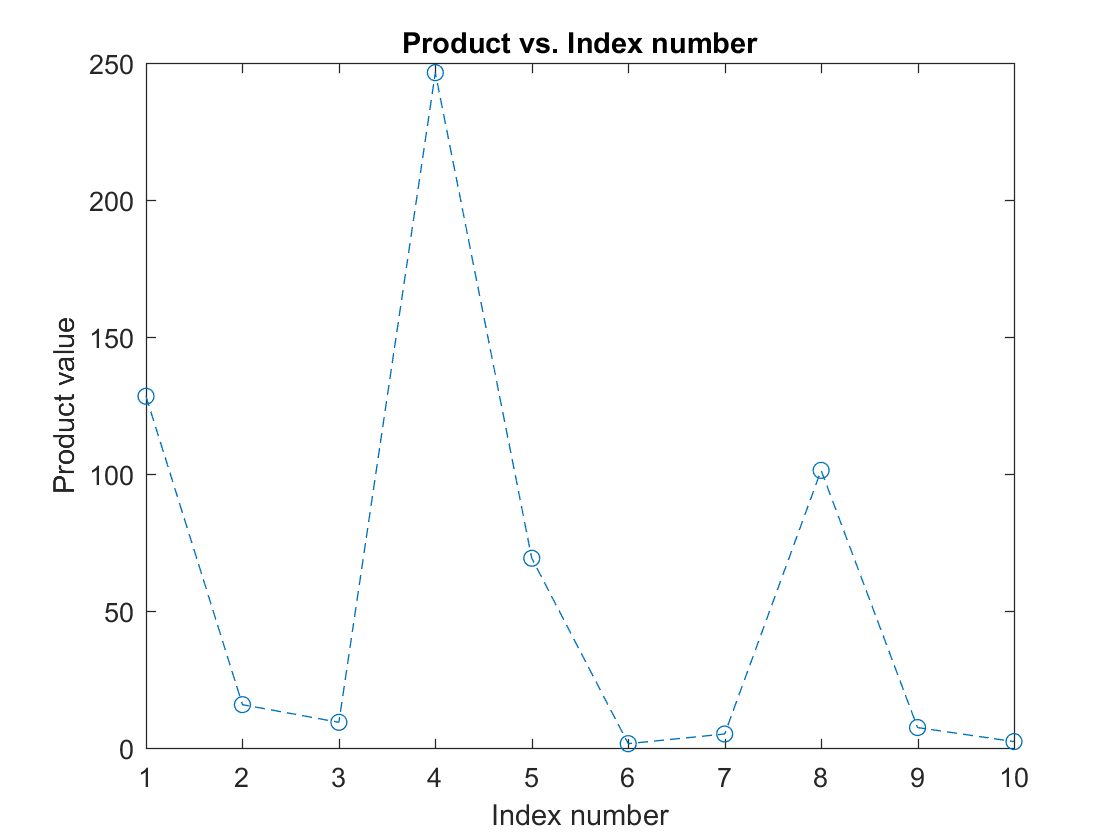
\includegraphics [width=4in]{exercise02_01.eps}



\end{document}
    
